\documentclass{standalone}
\usepackage{tikz}

\begin{document}
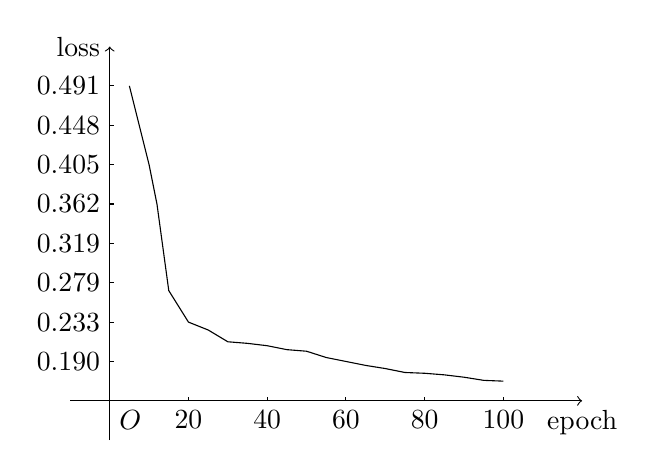
\begin{tikzpicture}
\draw[->](-.5,0)--(0, 0)node[below right]{$O$}--(1, 0)node[below]{$20$}--(2, 0)node[below]{$40$}--(3, 0)node[below]{$60$}--(4, 0)node[below]{$80$}--(5, 0)node[below]{$100$}--(6,0)node[below]{epoch};
\draw[->](0, -.5)--(0, 4.5)node[left]{loss};
\foreach\i in {1,...,5}{
    \draw (\i,0)--(\i,0.05);
}
\foreach\i/\j in {.5/0.190,1/0.233,1.5/0.279,2/0.319,2.5/0.362,3/0.405,3.5/0.448,4/0.491}{
    \draw (0,\i)node[left]{$\j$}--(0.05,\i);
}
\draw plot coordinates {(.25,4) (.5,3) (.6,2.5) (.75,1.4) (1,1) (1.25, .9) (1.5,.75) (1.75,.73) (2,.7) (2.25, .65) (2.5,.63) (2.75,.55) (3,.5) (3.25,.45) (3.5,.41) (3.75,.36) (4,.35) (4.25,.33) (4.5,.30) (4.75,.26) (5,.25)};
\end{tikzpicture}
\end{document}